\documentclass[13pt,titlepage]{article}

\usepackage[ngerman]{babel}
\usepackage[utf8]{inputenc}
\usepackage{color, colortbl}
\usepackage[table,xcdraw]{xcolor}
\usepackage{graphicx}
\usepackage{float}
\restylefloat{table}
\usepackage{verbatim}
\usepackage{hyperref}
\usepackage [backend=biber]{biblatex}

\addbibresource{sources.bib}

\usepackage[left=3cm,
  right=2cm,
  top=2.5cm,
  bottom=2cm,
  ]{geometry}

\def\code#1{\texttt{#1}}

\bibliography{sources.bib}

\begin{document}


\section*{Design für Demontage}
Sound Barrier, Inc., muss entscheiden, welches von zwei verschiedenen Lautsprecher-Designs umweltfreundlicher ist.
\paragraph{\textbf{ANSATZ} $\triangleright$ } Das Designteam erfasste folgenden Informationen für die zwei Audioanlagen-Designs, den Harmonizer und den Rocker:
\begin{itemize}
\item[1] Wiederverkaufswert der Komponenten minus der Transportkosten zur Demontage
\item[2] Einnahmen aus dem Wiederverwertung
\item[3] Bearbeitungskosten bzgl. der Demontage, Sortierung, Reinigung und Verpackung
\item[4] Entsorgungskosten, einschließlich Transport, Gebühren, Steuern und Bearbeitungszeit
\end{itemize}

\paragraph{\textbf{LÖSUNG $\triangleright$}} Das Designteam entwickelte die folgende Einnahmen- und Kosteninformationen für die Designvarianten. Alle folgenden Kennzahlen sind in der Einheit GE angegeben.


\paragraph{Harmonizer} $~$
\begin{table}[H]
\centering
\begin{tabular}{|l|c|c|c|c|}
\hline
\rowcolor[HTML]{343434} 
{\color[HTML]{FFFFFF}\scriptsize TEIL} & {\color[HTML]{FFFFFF} \begin{tabular}[c]{@{}c@{}}\scriptsize WIEDERVERKAUFS-\\ \scriptsize WERT / STÜCK\end{tabular}} & {\color[HTML]{FFFFFF} \begin{tabular}[c]{@{}c@{}}\scriptsize EINNAHMEN AUS\\ \scriptsize RECYCLING / STÜCK\end{tabular}} & {\color[HTML]{FFFFFF} \begin{tabular}[c]{@{}c@{}}\scriptsize BEARBEITUNGS-\\ \scriptsize KOSTEN / STÜCK\end{tabular}} & {\color[HTML]{FFFFFF} \begin{tabular}[c]{@{}c@{}} \scriptsize ENTSORGUNGS-\\ \scriptsize KOSTEN / STÜCK\end{tabular}} \\ \hline
Platine & 5,93 GE & 1,54 GE & 3,46 GE & 0,00 GE \\ \hline
\begin{tabular}[c]{@{}l@{}}Laminierte\\ Rückwand\end{tabular} & 0,00 & 0,00 & 4,53 & 1,74 \\ \hline
Spule & 8,56 & 5,65 & 6,22 & 0,00 \\ \hline
Prozessor & 9,17 & 2,65 & 3,12 & 0,00 \\ \hline
Rahmen & 0,00 & 0,00 & 2,02 & 1,23 \\ \hline
\begin{tabular}[c]{@{}l@{}}Gehäuse aus\\ Aluminium\end{tabular} & 11,83 & 2,10 & 2,98 & 0,00 \\ \hline
Gesamt & 35,49 GE & 11,94 GE & 22,33 GE & 2,97 GE\\ \hline
\end{tabular}
\end{table}


\paragraph{Rocker} $~$
\begin{table}[H]
\centering
\begin{tabular}{|l|c|c|c|c|}
\hline
\rowcolor[HTML]{343434} 
{\color[HTML]{FFFFFF} \scriptsize TEIL} & {\color[HTML]{FFFFFF} \begin{tabular}[c]{@{}c@{}}\scriptsize WIEDERVERKAUFS-\\ \scriptsize WERT / STÜCK\end{tabular}} & {\color[HTML]{FFFFFF} \begin{tabular}[c]{@{}c@{}}\scriptsize EINNAHMEN AUS\\ \scriptsize RECYCLING / STÜCK\end{tabular}} & {\color[HTML]{FFFFFF} \begin{tabular}[c]{@{}c@{}}\scriptsize BEARBEITUNGS-\\ \scriptsize KOSTEN / STÜCK\end{tabular}} & {\color[HTML]{FFFFFF} \begin{tabular}[c]{@{}c@{}}\scriptsize ENTSORGUNGS-\\ \scriptsize KOSTEN / STÜCK\end{tabular}} \\ \hline
Platine & 7,88 GE & 3,54 GE & 2,12 GE & 0,00 GE \\ \hline
Spule & 6,67 & 4,56 & 3,32 & 0,00 \\ \hline
Prozessor & 8,45 & 4,65 & 3,43 & 0,00\\ \hline
Rahmen & 0,00 & 0,00 & 4,87 & 1,97\\ \hline
\begin{tabular}[c]{@{}l@{}}Gehäuse aus\\ Plastik\end{tabular} & 0,00 & 0,00 & 4,65 & 3,98\\ \hline
Gesamt & 23,00 GE & 12,75 GE & 18,39 GE & 5,95 GE \\ \hline
\end{tabular}
\end{table}

\begin{center}
\noindent Mit Hilfe der Gleichung (S5-1) kann das Designteam die beiden Designoptionen vergleichen:
\linebreak
\linebreak 
\textit{Erlösrückgewinn = Wiederverkaufswert + Einnahmen aus Recycling
\linebreak
\hspace*{35mm} – Bearbeitungskosten – Entsorgungskosten (S5-1)}
\linebreak
\linebreak 
\textit{Erlösrückgewinn für Hamonizer = \$35.49 + \$11.94 - \$22.33 - \$2.97 = \$22.13 }
\linebreak
\textit{Erlösrückgewinn für Rocker = \$23.00 + \$12.75 - \$18.39 - \$5.95 = \$11.41}
\end{center}

\paragraph{\textbf{\"UBERBLICK $\triangleright$}} Nach Analyse der umweltbezogenen Einnahmen- und Kostenkomponenten jedes Lautsprecherdesigns gelangt das Designteam zu dem Urteil, dass der Harmonizer die geeignetere umweltfreundliche Designalternative ist, da er eine höhere Einnahmequelle bietet. Beachten Sie, dass das Team davon ausgeht, dass beide Produkte die gleiche Marktannahme, Rentabilität und Umweltfreundlichkeit aufweisen.
\paragraph{\textbf{\"UBUNGSAUFGABE $\triangleright$}} Was würde passieren, wenn es eine Anpassung in der Lieferkette gäbe, durch welche sich die Verarbeitungs- und Entsorgungskosten für die laminierte Rückwand des Harmonizers verdreifachen würden? [Antwort: Die Rückeinnahmen aus dem Harmonizer sind \$35.49 + \$11.94 - \$31.39 - \$6.45 = \$9.59. Dies liegt unter den Einnahmen des Rockers in Höhe von \$11,41, wodurch der Rocker zur umweltfreundlichen Designalternative wird, da er eine höhere Einnahmequelle bietet.]

\paragraph{\textbf{VERWANDTE PROBLEME $\triangleright$}} x S5.1, S5.2, S5.3, S5.9, S5.12, S5.13, S5.14

\section*{Weitere Designkonzepte im Fallbeispiel} 
Der Elektronikhersteller Regularsoft hat eine neue Taskforce gegründet, zur Analyse von alternativen Produktdesigns für sein Produktportfolio, bestehende aus Smartphones, Tablet, Notebooks und anderen technischen Geräten für den digitalen Arbeitsplatz. Grundlage für diese Entscheidung ist der globale Anstieg im Verbrauch von Kupfer und anderen Rohstoffen, welche essenziell für die einzelnen Komponente des Produktportfolios sind. Daneben wird auch innerhalb großer Teile der Kundengruppe von Regularsoft die Forderung nach umweltfreundlichen Produkten stärker. Mittlerweile nutzen einige Kunden kostengünstigere und umweltfreundlichere Alternativen der Konkurrenz. Vor allem im Bereich Smartphones und Notebook.
Mit den Ergebnissen der Taskforce will der Elektronikhersteller die ersten strategischen Schritte setzen, um seine Langzeitziel eines CO2-neutralen Unternehmens zu erreichen.


\paragraph{\textbf{BETRIEBLICHE KENNZAHLEN $\triangleright$}}
Für die Strategiefindung der Taskforce stellen die betrieblichen Kennzahlen der Regularsoft GmbH wichtige Grundsätze. Das Unternehmen konnte das letzte Geschäftsjahr mit folgenden Kennzahlen am 31.12.2020 abschließen:
\begin{itemize}
\item[•] Bilanzsumme (Mio. GE):		721,80
\item[•] Kapital (Mio. GE):			153,10
\item[•] Gesamtumsatz (Mio. GE):	980,40
\item[•] Jahresüberschuss (Mio. GE):	216,67
\end{itemize}
Für das angebrochen Geschäftsjahr hat der Finanzausschuss ein Jahreskapital von 14,6  Mio. GE für die Abteilung Marketing freigegeben. Außerdem wurden im Bereich Forschung \& Entwicklung 600 neue Mitarbeiter eingestellt und 80 weitere für die Vertriebsgruppen des Unternehmens.

\paragraph{\textbf{SONSTIGE KENNZAHLEN $\triangleright$}}
Im Rahmen der jährlicher interner und externer Untersuchungen haben sich des Weiteren folgende Ergebnisse zur Marktposition der Regularsoft ergeben:
\begin{itemize}
\item[•] \textbf{Nachfrage der Geräte:}
Umfragen bei Kunden ergaben, dass 91\% aller Neukunden auch für weitere Technikanschaffungen sich für Regularsoft-Produkte entscheiden würden. Bei Bestandskunden liegt diese Zahl sogar bei 95\%. Darüber hinaus gaben annähernd 75\% aller Geschäftskunden, so wie 81\% aller Privatkunden an, dass sie mit der Qualität der Produkte zufrieden sind und Regularsoft als Hersteller weiterempfehlen würden. Bereits in der Vergangenheit zeigte sich, dass die Nachfrage selbst bei kontroversen Produktneuerungen nur minimale fiel, aber im weiteren Zeitverlauf sich stabilisierte oder wieder anstieg.
\item[•] \textbf{Nachfrage des Betriebssystem:}
Das Betriebssystem von Regularsoft für Smartphones, Century-OS, belegt mit einem Marktanteil von 15,7\% den dritten Platz im globalen Markt. Dabei verwenden sowohl Firmen als auch privat Personen Century-OS als Betriebssystem für die betrieblichen, bzw. privaten Mobilgeräte. Innerhalb von Deutschland besitzt laut Marktforschungen jeder fünfte Haushalt ein mobiles Endgerät mit dem Century-OS.
\end{itemize}

\paragraph{\textbf{L"OSUNGANS"ATZE $\triangleright$}}
Während der Untersuchung haben sich zwei konkrete Konzepte für umweltfreundliche Produktdesigns hervorgehoben. 
\begin{itemize}
\item[•] \textbf{Modulares Produktdesign:}
Modularität im Design von Produkten definiert den Aufbau eines Produktes so, dass jede Komponente auf struktureller Sichtweise selbstständig sind und nur über bestimmte Schnittstellen verbunden sind. Dadurch wird eine dauerhafte Verbindung unter den Komponenten vermieden. Dies ermöglicht es einzelne Bestandteile einfacher aus einem Gerät zu entfernen und somit auszutauschen oder zu reparieren \cite{mp}. Für die Nutzer der Geräte öffnet dies auch die Möglichkeit selbständig Komponenten eines Geräts auszutauschen, ohne dabei zu Techniker oder Partnerunternehmen der Hersteller gehen zu müssen. Jedoch setzt diese Funktion in manchen Fällen technische Grundkenntnisse und eine kleine Ausstattung an Werkzeug zur die Lösung der Befestigungen voraus. Wobei es dabei lediglich um Standardwerkzeug wie z.B. Schraubenziehern handelt. Im Smartphone und Tablet Bereich haben bereits mehrere Kleinunternehmen innerhalb den letzten Jahren Geräte mit modularen Design an den Markt gebracht. Für die Hersteller solcher Produkte bietet sich durch die offenen Architektur der Produkte die Möglichkeit periodisch neuer Hardwarekomponenten zu entwickeln und den Kunden als Upgrade-Varianten anzubieten \cite{modest}. Somit lässt sich die Nutzungsdauer erhöhen, ohne dass die Geräte schnell technisch veralten und senkt aufgrund der verringerten Produktion von neuen Modellen die Umweltbelastung eines Unternehmens. Des Weiteren können die wertvollen Rohstoffe alter und nicht mehr genutzter Komponenten leicht recycelt werden.\\
\item[•] \textbf{Langlebige Software:}
Der Begriff "langlebige Software" beschreibt Betriebssysteme bzw. Anwendungen, welche durch spezielle, modulare Architekturen und erweiterten Support eine überdurchschnittliche Nutzungsdauer aufweisen können. Ziel dieser langlebigen Software ist es, auch ältere Geräte mit teilweise schwacher Hardware weiterhin unterstützen zu können und dadurch auch die Gesamtnutzungsdauer des Produktes zu verlängern. Erreicht wird die verlängerte Nutzungsdauer durch eine Maximierung der Kompatibilität bezüglich der Hardware, aber auch durch Transparenz gegenüber dem Benutzer. D.h. es wird genau kommuniziert, welche Änderungen ein Update zu Folge hat und der User kann frei entscheiden, ob er dieses durchführen oder ggf. auf eine ältere Softwareversion zurückkehren will. Die verwendeten modularen Architekturen ermöglichen dabei eine einfache Anpassung der Software an die Leistung der vorliegenden Hardware. Neue, ressourcenintensive Funktionen können auf diese Weise bei der Installation ausgelassen werden, während das Endgerät dennoch mit den aktuellen Sicherheits- und Kompatibilitätsupdates versorgt werden kann. Da in der Regel ein Ungleichgewicht zwischen potentieller Nutzungsdauer der Hardware und Nutzungsdauer der Software besteht, ist es mit dem Einsatz langlebiger Software möglich das Verhältnis der beiden Aspekte zu optimieren und somit sozusagen einen besseren Wirkungsgrad der Produkte zu erzielen.\\
Profitieren von dieser Praktik tut einerseits der Endkunde, da das Gerät in längeren Abständen ersetzt werden muss, was den Kunden wiederum dazu bewegen kann mehr Geld zu investieren, auf der anderen Seite profitiert auch die Natur, da längere Nutzungszyklen gleichzeitig weniger Elektroschrott bedeuten. 
\end{itemize}

\newpage
\paragraph{\textbf{SWOT-ANALYSE DER LÖSUNGSANSÄTZE  $\triangleright$}}
Nach Untersuchung beider Lösungs- ansätze hat die Regularsoft entschieden beide Varianten zu nutzen und sie als Basis für die nächsten Generationen des Produktportfolios anzuwenden. Somit kann Regularsoft sich lange Zeit für die Entwicklung der darauffolgenden Generationen konzentrieren und die Nachfrage durch modulare Upgrades beibehalten. Mit den Neuerungen kann das Unternehmen auch einige Materialien in den alten Komponenten recyceln. Grundlage für diese Entscheidung war folgende SWOT-Analyse der Taskforce:\\

\begin{figure}[h]
 \centering
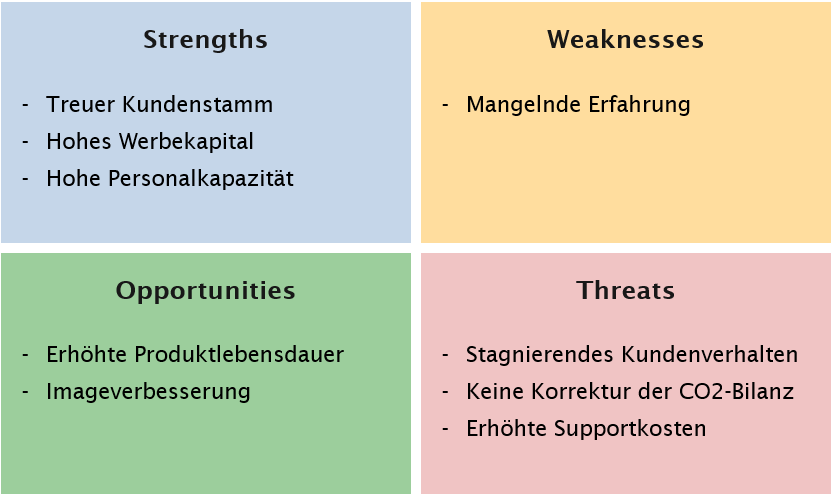
\includegraphics[width=0.9\textwidth]{SWOT}
 \caption{SWOT-Analyse zur Anwendung der neuen Designkonezpe}
 \label{fig:SWOT-Analyse}
\end{figure}

\paragraph{STÄRKEN}
\begin{itemize}
\item[•] \textbf{Treuer Kundenstamm:} 
Mit der hohen Kundezufriedenheit von 75\% bei Geschäfts- kunden und 81\% bei Privatkunden, so wie der stetig wachsenden Nachfrage nach Geräten der Marke Regularsoft und dem Vertrauen der Kunden, ist das Unternehmen bereit die Umstellung auf langlebiger Software und Modularität im Design zu nehmen.
\item[•] \textbf{Hohes Werbekapital:} 
Durch das zugewiesene Kapital  von 14,6 Mio. GE steht der Marketingabteilung des Unternehmens ausreichend finanzielle Mittel zur Verfügung, um die Produkte mit umweltfreundlicherem Design und Software stark zu vermarkten, um auch die Kunden auf die Neuerungen anzuziehen.
\item[•] \textbf{Ausreichend Personal:}
Auch an Personal fehlt es dem Unternehmen nicht. Sowohl für eine schnelle Entwicklung, als auch Vertrieb der nächsten Produktreihe stehen mit den global 600 neuen Entwicklungsmitarbeitern und 80 neuen Vertrieblern genügend Fachkräfte bereit.
\end{itemize}

\paragraph{SCHWÄCHEN}
\begin{itemize}
\item[•] \textbf{Mangelnde Erfahrung:}
Für beide Designkonzepte der Regularsoft ausreichend Erfahrung für eine schnelle Entwicklungszeit. Da bisher jegliche Software der Regularsoft mit dem traditionellen monolithischen Ansatz entwickelt wurde, konnte bis jetzt kein Know-how im Bereich der Entwicklung von modularer Software z.B. durch Microservices gesammelt werden. Ebenso sind viele technischer mit modularen Produktkonzepten noch unerfahren. Der Aufbau des erforderlichen Wissens und die Umsetzung der entsprechenden Konzepte erfordern immense Einarbeitungszeiten bei allen beteiligten Mitarbeitern.
\end{itemize}

\paragraph{CHANCEN}
\begin{itemize}
\item[•] \textbf{Erhöhte Produktlebensdauer:}
Mit den Varianten der modularen Hardwareaufbaus, als auch der Software zur Unterstützung der Hardwarekomponenten lässt sich die Lebensdauer eines einzelnen Geräts deutlich erhöhen \cite{mpd}. Während austauschbare Hardwareupgrades die Nachfrage der Kunden beibehalten und auch defekte Einheiten austauschen lässt, erreicht die langlebigerer Software, dass zwischen den Lebensdauern von Hard- und Software ein gesundes Gleichgewicht herrscht.

\item[•] \textbf{Imageverbesserung:}
Mit langlebigerer Software und Modularität als Basis der Produkte, kann Regularsoft aufgrund der gesteigerten Langlebigkeit der Produkte, dem zugänglicheren Recycling der Grundmaterialien und der insgesamt geringen Umweltbelastung, sein Firmenimage verbessern und sich umweltfreundliches und hochtechnologische Unternehmen auf den Markt positionieren. Mit Verbesserung des  grünen Images, werden auch alternative Kundengruppen die Produkte von Regularsoft in Betracht ziehen.
\end{itemize}

\paragraph{RISIKEN}
\begin{itemize}
\item[•] \textbf{Stagnierende Nachfrage:}
Damit die Umstellung umweltfreundliche Produkte erfolgreich ist, müssen vor allem die Kunden auf die Neuerungen anspringen. Kundengruppen, die jährlich neue Geräte anschaffen, könnte das Upgrade-Konzept abschrecken oder gar nicht interessieren. Währenddessen werden viele Nutzer davor zurückschrecken selbst Änderungen an Hardware vorzunehmen. Jedoch kann dies durch Upgrade-Angebote durch örtliche Filialen ausgeglichen werden. Trotzdem müssen die Kunden von Regularsoft ihr Kaufverhalten anpassen. Dieser Wandel wird längere Zeit benötigen und möglicherweise anfangs eine stagnierende Nachfrage mit sich ziehen.
\item[•] \textbf{Keine Korrektur der CO2-Bilanz:}
 Eine stagnierende Nachfrage kann jedoch auch auf die Umweltbelastung Auswirkungen haben. Zwar ermöglicht das neue Produktdesign einfacheres und besseres Recycling der verbauten Rohstoffe, jedoch kann auch eine optimales Recyclingkonzept nur zwischen 10-20\% CO2 der ursprünglichen Produktionsausstöße reduzieren \cite{mp}. Die Umweltbelastung wird daher nur erhöht, wenn Kunden die gesteigerte Produktlebensdauer voll ausnutzen.
\item[•] \textbf{Erhöhte Supportkosten:}
Durch die längere Unterstützung von Software und deren älteren Versionen auf immer älteren Geräten fallen im Vergleich zur aktuellen Situation erheblich höhere Supportkosten an. Da zum aktuellen Zeitpunkt nicht abgeschätzt werden kann, wie sich die langlebigere Software auf das Verhalten der Kunden auswirken wird, ist es folglich nicht möglich abzuschätzen, wie lange der Support für die jeweiligen Versionen der Betriebssysteme garantiert werden muss. Dies kann in im ungünstigen Fall zu unerwartet hohen Supportkosten führen.
\end{itemize}

\section*{Produktion Prozess}
Hersteller suchen nach Möglichkeiten, die Menge an Ressourcen im Produktionsprozess zu redu-zieren. Die Möglichkeiten zur Reduzierung der Umweltbelastung während der Produktion drehen sich zumeist um die Faktoren Energie, Wasser und Umweltverschmutzung. Einsparungen von Ener-gie und Verbesserung der Energieeffizienz entstehen durch den Einsatz alternativer Energien und energieeffizienterer Maschinen.  Beispielsweise:
\begin{itemize}
\item[•] S.C. Johnson baute ein eigenes Kraftwerk, das mit Erd- und Methangas aus einer nahen gele-genen Mülldeponie versorgt wird, wodurch die Abhängigkeit von Kohlekraftwerken verringert wurde.
\item[•] PepsiCo entwickelte Resource Conversation (ReCon), ein Diagnosetool zum Verständnis und zur Reduzierung des innerbetrieblichen Wasser- und Energieverbrauchs.  In den ersten zwei Jahren half ReCon Produktionsanalgen weltweit, 2,2 Milliarden Liter Wassereinsparungen zu erzielen, mit entsprechenden Kosteneinsparungen von fast 2,7 Millionen Dollar.
\item[•] Der Fast-Food-Hersteller Frito-Lay beschloss, Wasser aus Kartoffeln zu gewinnen, die zu 80\% aus Wasser bestehen. Jährlich werden in einer einzelnen Fabrik 350.000 Tonnen Kartoffeln zur Produktion von Kartoffelchips verwendet. Nach Verarbeitung der Kartoffeln, nutzt das Unter-nehmen das extrahierte Wasser wieder für die tägliche Produktion der jeweiligen Fabrik.
\end{itemize}

\noindent Durch derartige und vergleichbare Fortschritte im Produktionsprozess werden sowohl Kosten als auch Umweltbelastungen gesenkt. Dabei wird weniger Energie verbraucht, und es enden deutlich weniger Rohstoffe auf Mülldeponien.

\section*{Logistik}
Während sich Produkte durch die Lieferkette bewegen, bemühen sich Betriebsleiter um effiziente Routen- und Liefernetzwerke, genau wie sie anstreben, die Betriebskosten zu senken. Hierdurch wird die Umweltbelastung reduziert. Management-Analysetechniken (wie lineare Programmie-rung, Software für Warteschlangen und Fahrzeugrouting) helfen Firmen weltweit bei der Optimie-rung durchdachter Lieferketten- und Distributionsnetzwerke. Netzwerke von Containerschiffen, Flugzeugen, Zügen und LKWs werden ausgewertet, um die Anzahl der zurückgelegten Meilen oder die benötigte Stundenzahl für Lieferungen zu reduzieren. Beispielsweise:
\begin{itemize}
\item[•] Der Versanddienstleister UPS hat festgestellt, dass Linkskurven die Lieferzeit verlängern. Dies wiederum erhöht den Treibstoffverbrauch und die CO2-Emissionen. Daher konzipiert UPS sei-ne Lieferrouten mit möglichst wenigen Linkskurven. In ähnlicher Weise fliegen Flugzeuge in verschiedenen Höhelagen und Flugrouten, um günstigere Windkonditionen zu nutzen und so den Treibstoffverbrauch und die CO2-Emissionen zu reduzieren.
\item[•] Lebensmittelhersteller verfügen mittlerweile über Lastwagen mit drei Temperaturzonen (gefroren, gekühlt und ungekühlt), anstatt wie früher für jede Warenart einen eigenen Fahrzeug-typ einzusetzen.
\item[•] Das Unternehmen Whirlpool hat seine Verpackung radikal überarbeitet, um "Beulen und Dellen" an Geräten bei der Lieferung zu vermeiden und konnte dadurch enorme Einsparungen bei den Transport- und Garantiekosten erzielen.
\end{itemize}

\noindent Zur weiteren Verbesserung der logistischen Effizienz evaluieren die Betriebsleiter ebenfalls Ausrüstungsalternativen unter Berücksichtigung der Kosten, der Amortisationsdauer und der vom Unternehmen festgelegten Umweltziele. Beispiel S2 befasst sich mit der Entscheidungsfindung unter Betrachtung der Life-Cycle-Ownership-Kosten. Ein Betrieb muss entscheiden, ob er mehr im Voraus für umweltfreundliche Fahrzeuge zahlt, um seine Nachhaltigkeitsziele zu erreichen, oder ob er weniger im Voraus für Fahrzeuge ausgibt, welche die Ziele nicht unterstützen.

\section*{Beispiel S2: Life-Cycle-Ownership und Crossover-Analyse}
Blue Star startet einen neuen Vertriebsservice, der Autoteile an die Serviceabteilungen regionaler Autohändler liefert. Blue Star hat zwei Kleinlaster gefunden, welche für die Aufgabe geeignet wären, und muss nun einen auswählen, um diesen neuen Service anbieten zu können. Der Ford Tri-Van, erhältlich für 28.000 GE, verwendet normales bleifreies Benzin mit einer durchschnittlichen Kraftstoffeffizienz von 24 Meilen pro Gallone. Die Betriebskosten des TriVan belaufen sich auf  0,20 GE pro Meile. Der CityVan, ein Hybrid-Lkw, kostet in der Anschaffung 32.000 GE und verbraucht normales bleifreies Benzin und Batterieantrieb, er erreicht durchschnittlich 37 Meilen pro Gallone. Die Betriebskosten des CityVan belaufen sich auf 0,22 GE pro Meile. Die jährlich zurückgelegte Stre-cke wird auf ca. 22.000 Meilen geschätzt, wobei die Lebensdauer der beiden Fahrzeuge auf 8 Jahre geschätzt wird. Der durchschnittliche Benzinpreis beträgt 4,25 GE pro Gallone.

\paragraph{\textbf{ANSATZ} $\triangleright$ }
Blue Star wendet Gleichung (S5-2) an, um die Gesamtlebenszykluskosten für jedes Fahrzeug zu bewerten:
Gesamtlebenszykluskosten = Kosten des Fahrzeugs + Lebenszykluskosten des Kraftstoffs + Lebenszyklus-Betriebskosten (S5-2)\\
a) Welches Modell ist, basierend auf den Lebenszykluskosten, die beste Wahl?\\
b) Wie viele Meilen m\"ussen gefahren werden, damit bei beiden Lastw\"agen Kostengleichheit herrscht?\\
c) Nach wie vielen Jahren wird der Break-Even-Point erreicht?

\paragraph{\textbf{LÖSUNG} $\triangleright$ }\mbox{}\\

a) \\\mbox{}\\
Ford TriVan:\\

$$ Gesamtlebenszykluskosten = \$28000 +(\frac{22000\frac{Meilen}{Jahr}}{24 \frac{Meilen}{Gallone}}) \cdot (\$4.25/Gallone) \cdot (8 \ Jahre)$$ \\ $$+ 22000 \frac{Meilen}{Jahr} \cdot  (\$0.20/Meile) \cdot  (8 \ Jahre) = \$28000 + \$31167 + \$35200 = \$94367$$\\
\mbox{}
\\

 Honda CityVan:\\
$$ Gesamtlebenszykluskosten = \$32000 +(\frac{22000\frac{Meilen}{Jahr}}{37 \frac{Meilen}{Gallone}}) \cdot (\$4.25/Gallone) \cdot  (8 \ Jahre) $$\\$$+ 22000 \frac{Meilen}{Jahr} \cdot  (\$0.22/Meile) \cdot  (8 \ Jahre) = \$32000 + \$20216 + \$38720 = \$90936$$\\
 
 b) Der Break-Even Point sei \emph{M} in Meilen, beide Gleichungen zu den Lebenszykluskosten werden gleichgesetzt und anschließend nach \emph{M} gel\"ost:\\
 
 Gesamtkosten für Ford Trivan = Gesamtkosten f\"ur Honda CityVan\\
 
 $$ \$28000 +  [ \frac{4.25\frac{\$}{Gallone}}{24\frac{Meilen}{Gallone}} + 0.20\frac{\$}{Meile}](\emph{M} \ Meilen) = \$32000 + [ \frac{4.25\frac{\$}{Gallone}}{37\frac{Meilen}{Gallone}} + 0.22\frac{\$}{Meile}](\emph{M} \ Meilen) $$\\
 oder,\\
 $$ \$28000 + (0.3770\frac{\$}{Meile})(\emph{M}) = \$32000 + (0.3349\frac{\$}{Meile})(\emph{M}) $$\\
 oder,\\
 $$ (0.0421\frac{\$}{Meile})(\emph{M}) = \$4000 $$\\
$$ \emph{M}=\frac{\$4000}{0.0421\frac{\$}{Meile}}=95012 Meilen $$\\

c) Der Break-Even Point in Jahren:

$$ Break-Even Point = \frac{95012 Meilen}{22000\frac{Meilen}{Jahr}} = 4.32 \ Jahre $$

\paragraph{\textbf{ERGEBNISSE} $\triangleright$ }\mbox{}\\


a) Trotz der h\"oheren Anschaffungs- und Betriebskosten pro Meile ist der Honda CityVan die bessere Wahl. Die Ersparnisse gegen\"uber dem Modell von Ford resultieren aus dem geringeren Spritverbrauch.\\

b) Der Break-Even Point befindet sich bei 95012 Meilen, was bedeutet, dass ab diesem Punkt beide Modelle die selben Kosten verursachen.\\

c) Es wird 4.32 Jahre dauern, bis sich die Kosten für den Kauf eines der beiden Fahrzeuge amortisiert haben. Dies ist der Punkt der Gleichgültigkeit zwischen den beiden Fahrzeugen. Allerdings wird es  Blue Star über die erwartete Lebensdauer von 8 Jahren etwa 0.03 Dollar pro Meile weniger kosten, anstatt des Fords den Honda zu betreiben.

\paragraph{\textbf{ÜBUNGEN} $\triangleright$ }
Was w\"aren die Gesamtlebenszykluskosten f\"ur jeden Van, der Break-Even Point in Meilen und der Break-Even Point in Jahren, sollte der Benzinpreis auf \$3.25 fallen? [Antwort: Kosten für Ford TriVan: \$87033; Kosten f\"ur Honda CityVan: \$86179; Break-Even Point in Meilen: 144927; Break-Even Point in Jahren: 6.59]

\paragraph{\textbf{ÄHNLICHE AUFGABEN} $\triangleright$ }
S5.4, S5.5, S5.6, S5.10, S5.11, S5.15, S5.16, S5.17, S5.18, S5.19


\section*{Beispiel S3}

Das Unternehmen Dominos startet einen neuen, auf Umweltverträglichkeit ausgelegten, Lieferdienst für Pizzabestellungen und benötigt für die Auslieferung neue Kleinwagen. Zur Auswahl steht jeweils ein Modell mit Elektroantrieb und eines mit Dieselmotor. Da das Dominos großen Wert auf Nachhaltigkeit und Umweltverträglichkeit legt, ist es wichtig, das Fahrzeug mit der geringsten Umweltbelastung zu wählen. Dazu soll analysiert werden, welches Fahrzeug im Anwendungszweck des Unternehmens den geringsten CO2 Ausstoß generiert.\\ Bei der Herstellung des Dieselfahrzeugs fallen 8300kg CO2 an, während die Herstellung des Elektrofahrzeugs 8000kg CO2 und die Fertigung dessen Batterie 8880kg (Herstellung in China), bzw. 5952kg (Herstellung in der EU) generiert \cite{vdi}. Gemäß dem aktuellen Strommix in Deutschland schlägt ein gefahrener Kilometer mit dem E-Auto mit 93g CO2 zu Buche \cite{vdi}. Bei dem Dieselfahrzeug berechnet sich dieser Wert aus dem durchschnittlichen Verbrauch, welcher mit 4.5l/100km angegeben ist \cite{vdi}, sowie des C02 Ausstoßes pro Liter Diesel, welcher sich auf 2.65kg/l beläuft \cite{diesel}. Weiterhin wird angenommen, dass die jährliche Fahrleistung 30000km beträgt und die Nutzungsdauer des Fahrzeugs bei sechs Jahren \cite{finanzministerium} liegt.  
\paragraph{\textbf{ANSATZ} $\triangleright$ }
Dominos verwendet die folgende Gleichung zur Ermittlung des gesamten CO2 Ausstoßes innerhalb der Nutzungsdauer: \\
$$Gesamtausstoß\ =\ Herstellung\ des\ Fahrzeugs\ +\ (Jahreslaufleistung\ \cdot\ CO2\ Ausstoß\ pro\ km)\ \cdot\ Nutzungsdauer$$\\
a) Welche Antriebsart ist bezogen auf den Umweltschutz für das Unternehmen die bessere Wahl?\\
b) Wie viele Kilometer müssen im Jahr gefahren werden, damit die CO2 Bilanz der beiden Fahrzeuge gleich ist?\\
c) Wie müsste die Nutzungsdauer angepasst werden, sodass sich die Auswahl des Antriebs verändert?\\

\paragraph{\textbf{LÖSUNG} $\triangleright$ }\mbox{}\\

a) \\\mbox{}\\
Dieselffahrzeug:\\

$$ Gesamtausstoß = 8300kg\ +\ (30.000km\ \cdot (\frac{4.5\frac{l}{100km}\ \cdot  2.65\frac{kg}{l}}{100km})\ \cdot  6\ Jahre $$\\ $$=\ 29765kg\ CO2-Ausstoß\ in\ der\ gesamten\ Nutzungsdauer$$ \\
\mbox{}
\\
Elektrofahrzeug mit Batterie aus China:\\

$$ Gesamtausstoß = 8880kg\ +\ 8000kg\ +\ (30000km\ \cdot  (0.093\frac{kg}{km})\ \cdot  6\ Jahre $$\\ $$=\ 33620kg\ CO2-Ausstoß\ in\ der\ gesamten\ Nutzungsdauer$$ \\
\mbox{}
\newpage

Elektrofahrzeug mit Batterie aus der EU:\\

$$ Gesamtausstoß = 5952kg\ +\ 8000kg\ +\ (30000km\ \cdot  (0.093\frac{kg}{km})\ \cdot  6\ Jahre $$\\ $$=\ 30692kg\ CO2-Ausstoß\ in\ der\ gesamten\ Nutzungsdauer$$ \\
\mbox{}
\\
b) Der Break-Even Point sei \emph{J} in Kilometern pro Jahr, beide Gleichungen zum Gesamtausstoß werden gleichgesetzt und anschließend nach \emph{J} gel\"ost:\\

Für ein Elektrofahrzeug mit Batterie aus China:\\
$$8880kg\ +\ 8000kg\ +\ J\ \cdot  0.093\frac{kg}{km}\ \cdot  6\ Jahre= 8300kg\ +\ J\ \cdot  \frac{4.5\frac{l}{100km}\ \cdot  2.65\frac{kg}{l}}{100km}\ \cdot  6\ Jahre $$\\
oder, \\
$$8880kg\ +\ 8000kg\ -\ 8300kg\ =\ J\ \cdot  \frac{4.5\frac{l}{100km}\ \cdot  2.65\frac{kg}{l}}{100km}\ -\ J\ \cdot  (0.093\frac{kg}{km}\ \cdot  6\ Jahre$$\\
oder,\\
$$J\ =\ \frac{8880kg\ +\ 8000kg\ -\ 8300kg}{\frac{4.5\frac{l}{100km}\ \cdot  2.65\frac{kg}{l}}{100km}\ -\ 0.093\frac{kg}{km}\ \cdot  6\ Jahre}\ \approx \ 54500\frac{km}{Jahr}$$
\\\mbox{}\\
Analog dazu bei einem Fahrzeug mit Batterie aus der EU:\\

$$J\ =\ \frac{5952kg\ +\ 8000kg\ -\ 8300kg}{\frac{4.5\frac{l}{100km}\ \cdot  2.65\frac{kg}{l}}{100km}\ -\ 0.093\frac{kg}{km}\ \cdot  6\ Jahre}\ \approx\ 35800\frac{km}{Jahr}$$\\

c) Erforderliche Nutzungsdauer, damit die Auswahl auf den Elektroantrieb fällt:\\
$$ Break-Even Point\ in\ Jahren\ =\ \frac{35800\frac{km}{Jahr}\ \cdot  6\ Jahre}{30000\frac{km}{Jahr}} = 7.16 \ Jahre $$\\

\paragraph{\textbf{ERGEBNISSE} $\triangleright$ }\mbox{}\\


a) Trotz des höheren CO2 Ausstoßes beim Betrieb des Dieselfahrzeugs, ist es (bezogen auf den CO2 Ausstoß) für Dominos die bessere Wahl. Aufgrund der hohen, in der Batterieproduktion generierten CO2 Belastung, kann sich das Elektrofahrzeug bei einer Jahreslaufleistung von 30000km nicht durchsetzen.\\

b) Der Break-Even Punkt befindet sich bei 54500km, bzw. 35800km pro Jahr. Ab diesem Punkt wäre der Elektroantrieb, dem Dieselmotor vorzuziehen.\\

c) Damit Dominos mit der Nutzung eines Elektrofahrzeugs umweltfreundlicher sein kann, als mit einem Dieselfahrzeug, müsste das Fahrzeug bei einer Jahreslaufleistung von 30000km mindestens für 7.16 Jahre verwendet werden
\section*{End-of-Life Phase}

Es wurde bereits erwähnt, dass Manager während des Produktdesigns bedenken müssen, was mit einem Produkt oder seinen Materialien geschieht, nachdem das Produkt das Ende seiner Lebensdauer erreicht hat. Produkte mit weniger Material, mit recyceltem Material oder mit wiederverwertbaren Materialien tragen alle zur Nachhaltigkeit bei und verringern die Notwendigkeit der Entscheidung "verbrennen oder vergraben" und erm\"oglichen die Schonung knapper natürlicher Ressourcen. Innovative und nachhaltigkeitsbewusste Unternehmen entwerfen heute geschlossene Lieferketten, auch Reverse Logistics genannt. Unternehmen können nicht mehr ein Produkt verkaufen und es dann vergessen. Sie müssen End-of-Life-Systeme für die physische Rückgabe von Produkten entwerfen und implementieren, die das Recycling oder die Wiederverwendung erleichtern.\\
Der Baumaschinenhersteller Caterpillar hat mit seinem Fachwissen über Wiederaufbereitungstechnologie und -prozesse Cat Reman, eine Wiederaufbereitungsinitiative, ins Leben gerufen, um ihr Engagement für Nachhaltigkeit zu zeigen. Caterpillar stellt Teile und Komponenten wieder her, die eine neuwertige Leistung und Zuverlässigkeit zu einem Bruchteil des Neupreises bieten und gleichzeitig die Auswirkungen auf die Umwelt reduzieren. Das Wiederaufbereitungsprogramm basiert auf einem Austauschsystem, bei dem Kunden eine gebrauchte Komponente im Austausch gegen ein wiederaufbereitetes Produkt zurückgeben. Das Ergebnis sind niedrigere Betriebskosten für den Kunden, weniger Materialabfall und ein geringerer Bedarf an Rohmaterial für die Herstellung neuer Produkte. In einem Zeitraum von einem Jahr hat Caterpillar 2.1 Millionen Altgeräte zurückgenommen und ca 59 Millionen Kilogramm recyceltes Eisen wiederaufbereitet.\\ Die Box OM in Aktion "Designing for End of Life" beschreibt die Designphilosophie von Apple, um die Demontage, das Recycling und die Wiederverwendung ihrer iPhones, die das Ende ihrer Lebensdauer erreicht haben, zu erleichtern.\\
Photovoltaik Anlagen sind ein weiterer Bereich, in dem zukünftig gutes End of Life Management betrieben werden muss. Ein Bericht, der von der Internationalen Agentur für Erneuerbare Energien (IRENA) zusammen mit dem Programm für photovoltaische Energiesysteme der Internationalen Energieagentur (IEA-PVPS) erstellt wurde, beschäftigt sich mit genau diesem Thema. Der Einsatz der Photovoltaik (PV) hat seit Anfang der 2000er Jahre mit beispielloser Geschwindigkeit zugenommen. Mit der Zunahme des globalen PV-Markts wird auch die Menge der stillgelegten PV-Paneele zunehmen, und bis Anfang der 2030er Jahre werden große Mengen an jährlichem Abfall erwartet. Der wachsende Abfall an PV-Panelen stellt eine neue ökologische Herausforderung dar, bietet aber auch nie dagewesene Möglichkeiten, Werte zu schaffen und neue wirtschaftliche Wege zu beschreiten. Laut diesem Bericht könne das Recycling oder die Wiederverwendung von PV-Solarpaneelen am Ende ihrer etwa 30-jährigen Lebensdauer bis 2050 weltweit einen geschätzten Bestand von 78 Millionen Tonnen an Rohstoffen und anderen wertvollen Komponenten freisetzen. Bei vollständiger Rückführung in die Wirtschaft könne der Wert des zurückgewonnenen Materials bis 2050 15 Milliarden USD übersteigen. Neben des wirtschaftlichen Vorteils ergibt sich auch ein immenser Nutzen für die Umwelt und ist für den weltweiten Übergang zu einer nachhaltigen und zunehmend auf erneuerbaren Energien basierenden Energiezukunft von wesentlicher Bedeutung.\cite{pv}


\newpage

\printbibliography

\end{document}
